\begin{figure}[!htb]
    \centering
    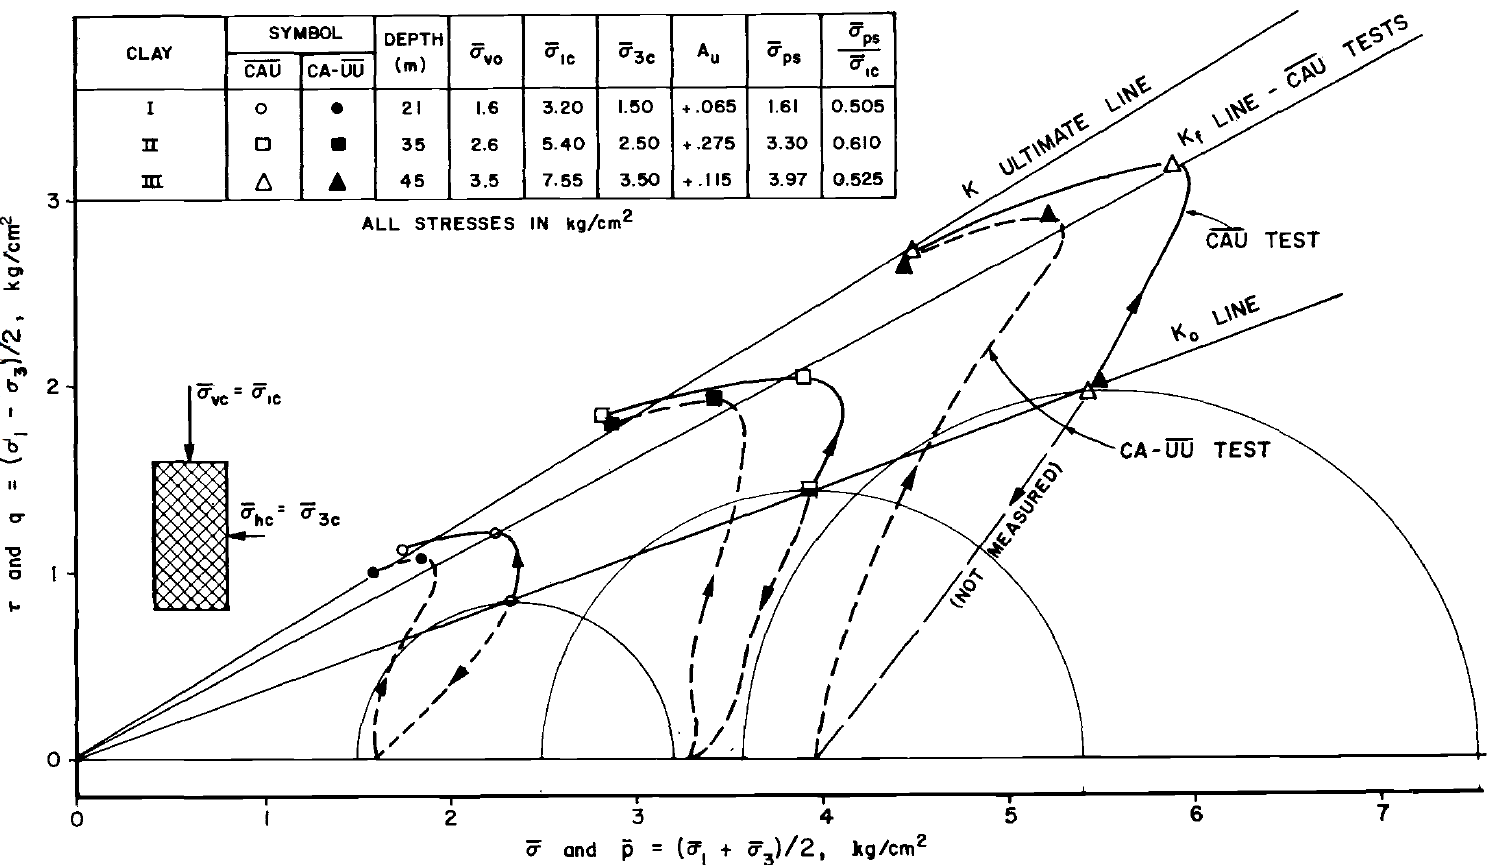
\includegraphics[width=0.8\textwidth]{figures/figure-2.png}
    \caption{Effect of Perfect Sampling on Stress Paths for Normally Consolidated Kawasaki Clays.}
    \addtocounter{figure}{-1}
    \vspace{-5pt}
    \renewcommand{\figurename}{图}
    \caption{完美采样对正常固结的川崎黏土应力路径的影响。}
    \renewcommand{\figurename}{Figure}
    \label{figure:2}
\end{figure}